\documentclass[12pt,letterpaper,noanswers]{exam}
\usepackage[usenames,dvipsnames,svgnames,table]{xcolor}
\usepackage[margin=0.9in]{geometry}
\renewcommand{\familydefault}{\sfdefault}
\usepackage{multicol}
\pagestyle{head}
\header{AM 111 Class 16}{}{Approximating integrals, p.\thepage}
\runningheadrule
\headrule
\usepackage{siunitx}
\usepackage{graphicx} % more modern
\usepackage{amsmath} 
\usepackage{amssymb} 
\usepackage{hyperref}
\usepackage{tcolorbox}
\usepackage{enumitem}
\usepackage{listings}
\def\mbf{\mathbf}
\newcommand{\vc}[1]{\boldsymbol{#1}}
\def\dsst{\displaystyle}
\DeclareMathOperator*{\argmin}{arg\,min} % thin space, limits underneath in displays
%\usepackage[numbered,autolinebreaks,useliterate]{mcode}

\begin{document}
 \pdfpageheight 11in 
  \pdfpagewidth 8.5in

\noindent 



\noindent\textbf{Big picture}

Today: Approximating $\int_W f dV$ for regions of integration with dimension higher than $1$.

\vspace{0.2cm}
\hrule
\vspace{0.2cm}

\noindent \textbf{Skill check practice}

The average value of $f$ at $1000$ randomly selected points in $W = [0,2]\times[0,2]\times[0,2]$ is $0.612$.  Write an expression for the Monte Carlo estimate of $\int_W f dV$.



\vspace{0.2cm}
\hrule
\vspace{0.2cm}

\noindent \textbf{Skill check solution}

The size of $W$ is $2^3 = 8$ so the estimate is $8*0.612$

\vspace{0.2cm}
\hrule
\vspace{0.2cm}




\subsection*{Monte Carlo integration }

(see Greenbaum and Chartier \S 3.3)



\subsection*{Why do we need Monte Carlo?}

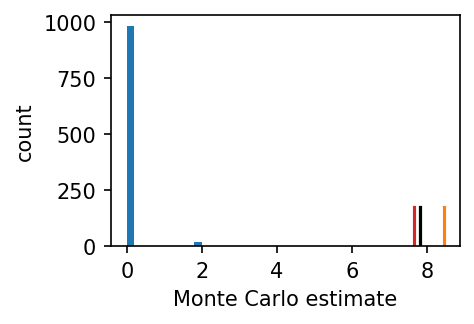
\includegraphics{AM111-F23-CourseNotes/img/C16-MC4pts.png}
     
\begin{enumerate}
\item $1000$ results of a four point Monte Carlo quadrature for $f(x) = e^x - 2\sin(4x) + 1$ are shown above.  Estimates using composite trapezoid, composite midpoint, and Gaussian quadrature are shown as vertical lines.  Approximate the proportion of Monte Carlo estimates that are worse than the worst deterministic quadrature rule.
\vspace{1in}

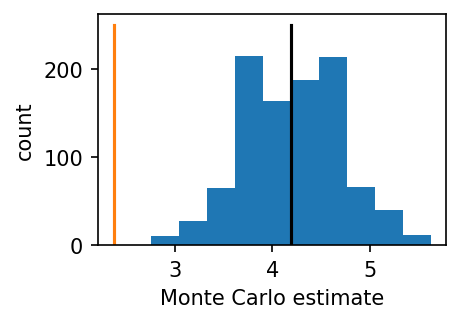
\includegraphics{AM111-F23-CourseNotes/img/C16-MC64pts.png}
\item $1000$ results of a four point in each dimension Monte Carlo quadrature are show above.  The exact value of the integral is in black and an estimate using the composite trapezoid rule is shown as a second vertical line.  Approximate the proportion of Monte Carlo estimates that are worse than the composite trapezoid rule.
\vspace{1cm}

\item In 1D the interval size, $h$, is inversely proportional to the total number of quadrature points, $M$.  $h = (b-a)/M$.

In the 3D case, assume an $n\times n\times n$ grid of points, with $M$ total points.  Write $n$ in terms of $M$.  $h$ is inversely proportional to $n$.  How does it relate to $M$?

\vspace{1.5in}

\end{enumerate}

%The 1D trapezoidal rule is 2nd order accurate: $I - I_T = \mathcal{O}(h^2)$.  In $d$ dimensions, it will be order $2/d$ instead.  For large dimensions $d$, this reduces accuracy substantially.  This is called the \textbf{curse of dimensionality}.

\subsection*{How do we compute a Monte Carlo integral?}

\begin{enumerate}[resume]
    \item Let $f(x,y) = \left\{\begin{array}{l} 1\text{ if } \sqrt{x^2+y^2}\leq 1 \\
    0 \text{ otherwise }
     \end{array}\right.$

    Working by hand, compute the integral of this function over the domain $[0,1]\times [0,1]$.

\vspace{1in}
    
     \item The average value of $f$ at $1000$ randomly selected points in $[0,1]\times [0,1]$ is $0.785$.

     Use this information to find a Monte Carlo estimate of the integral.  How does it compare to the exact value?

     \vspace{1in}

     \item How would you adjust $f$ if you wanted to integrate the function $e^x$ on the quarter disk, instead of the function $1$?

\vspace{1in}

\item 
For the following code
\begin{lstlisting}[basicstyle=\small,language=python]

import numpy as np
rng = np.random.default_rng()

def fc(x,y): 
    return x**2+y**2
    
npoints = 10000
xyvals = rng.uniform(0,2,[npoints,2])
f_avg = np.mean(fc(xyvals[:,0],xyvals[:,1]))
integral = 4*f_avg
\end{lstlisting}
\begin{parts}
\itemsep40pt
\item How many random points are being generated?  Are they points in $\mathbb{R}$?  $\mathbb{R}^2$?  $\mathbb{R}^3$?
\item What are the minimum and maximum values of the coordinates of the points?
\item What function is being evaluated on these points?
\item Set up a double integral that corresponds to the integral being approximated here.
\vspace{1in}
\end{parts}
\end{enumerate}




% 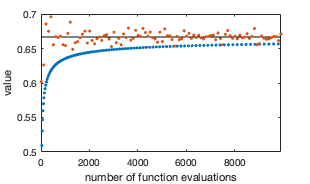
\includegraphics[width=0.45\textwidth]{img/C15MC.png}
% 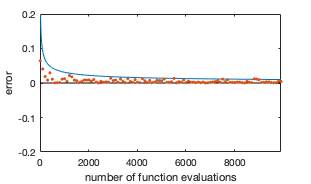
\includegraphics[width=0.45\textwidth]{img/C15MCerror.png}

\vspace{0.2cm}
\hrule
\vspace{0.2cm}


% \noindent\textbf{A non-unit interval}
% \begin{enumerate}[resume=classQ]
% \item \texttt{uniform(0,5,3)} generates an array of three random numbers uniformly spaced between $0$ and $5$.  \texttt{uniform(1,5)} generates a single random number uniformly spaced between $1$ and $5$.
    
% Write Python code to generate a pair of random numbers, with one between $-1$ and $1$ and the second between $2$ and $4$.
% \vspace{1in}
% \end{enumerate}
\eject
\begin{enumerate}[resume]
\item Consider the 3D region described by $xyz\leq 1$ and $-5\leq x,y,z\leq 5$.  Suppose we wish to find the volume of this region.  How would you do this via Monte-Carlo integration?  

Provide an outline of your code.
\vspace{3in}
\item How would your code change if you are finding the mass of the object and it has density $e^{0.5z}$, rather than finding the volume?
\vfill
\end{enumerate}
    

% \noindent\textbf{Approximating $\pi$}

% Consider the following code for Monte Carlo integration.
% \begin{lstlisting}   
% npoints = 10**6
% xyvals = uniform(0,1,[npoints,2])
% indomain = (xyvals[:,0]**2+xyvals[:,1]**2)<1
% integral = 4*sum(indomain)/npoints
% \end{lstlisting}
% \begin{enumerate}[resume=classQ]
% \item Answer the following questions about the code above.
% \begin{parts}
% \item What is the range of $x$ being used?  What about $y$?
% \vspace{1cm}

% \item What is the set of $(x,y)$ for which the function will be nonzero (so $x$ and $y$ are \texttt{indomain})
% \vspace{1cm}
% \item Identify the region of integration.
% \vspace{1cm}
% \item Given the final value is \texttt{4*sum(indomain)/npoints}, what is the function of integration?
% \end{parts}
% \end{enumerate}

%Let $f(x,y) = 4$.  Let $R$ be the region in the first quadrant where $x^2+y^2\leq 1$.  $\displaystyle\int_R f(x,y) dA = \int_0^{\pi/2}\int_0^1 4r\ dr\ d\theta = \pi$.

\subsection*{Error in Monte Carlo}

The standard deviation of the value of the integral is given by $\frac{V}{\sqrt{N}}\sigma_N$ where $V$ is the size of the region of integration and $\sigma_N$ is the standard deviation of $f$, the function of integration, over $N$ randomly generated points in the region.



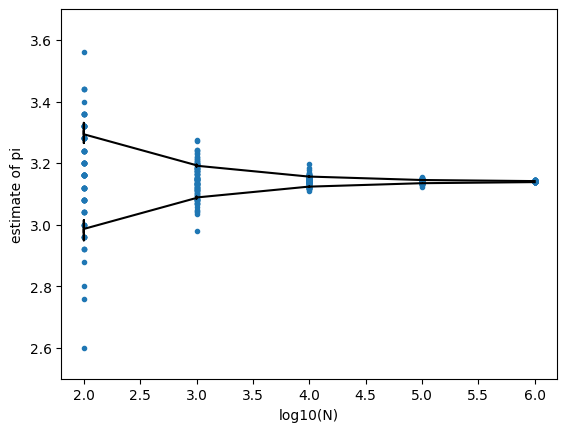
\includegraphics[width=0.5\linewidth]{img/C17piest.png}

The black curves in the figure above are $\pi + \frac{V}{\sqrt{N}}\sigma_N$ and $\pi - \frac{V}{\sqrt{N}}\sigma_N$

%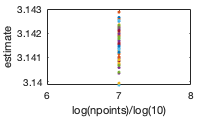
\includegraphics{img/C15MCpi7.png}
\vspace{0.1cm}

% \noindent\textbf{Circular region with non-uniform function}
% \begin{enumerate}[resume=classQ]
%     \item Approximate the integral of a function that is not uniform: let $f(x,y) = xy$.
    
%     \texttt{def fc(x,y): return x*y}
    
%     Let $R$ again be the region in the first quadrant where $x^2+y^2\leq 1$.
    

    
%     How would you modify the code at the top of the page to incorporate this nonuniform function?
% \end{enumerate}

% \vspace{1in}

% \noindent\textbf{Example}

% %\begin{tabular}{p{12cm} c }
% Provide pseudocode for using Monte-Carlo integration to approximate the area, $\int_R dA$, where $R$ is the crescent shape shown. %&

% 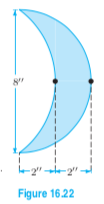
\includegraphics[scale=0.65]{img/C16crescent.png}
% %\end{tabular}



\end{document}